\documentclass[11pt]{article}
\usepackage[a4paper,margin=1in]{geometry}
\usepackage{booktabs}
\usepackage{tabularx}
\usepackage{graphicx}
\usepackage{float}
\usepackage[section]{placeins}
\usepackage{array}
\usepackage{amsmath}
\usepackage{xcolor}
\usepackage[hidelinks]{hyperref}
\usepackage{fancyhdr}
\usepackage[T1]{fontenc}
\usepackage{lmodern}

\definecolor{faissblue}{HTML}{1F4D78}
\pagestyle{fancy}
\fancyhf{}
\lhead{\textit{faissR} supplementary material}
\rhead{\thepage}
\setlength{\headheight}{14pt}
\setlength{\emergencystretch}{3em}
\renewcommand{\headrulewidth}{0.4pt}

\newcommand{\code}[1]{\texttt{#1}}
\newcommand{\pkg}[1]{\textsf{#1}}
\newcommand{\proglang}[1]{\textsf{#1}}
\newcommand{\class}[1]{\texttt{#1}}
\newcolumntype{Y}{>{\raggedright\arraybackslash}X}
\renewcommand{\thetable}{S\arabic{table}}
\renewcommand{\thefigure}{S\arabic{figure}}

\title{\textbf{Supplementary Material}\\[0.4em]
\large \pkg{faissR}: Nearest-Neighbor Search with FAISS and cuVS in R}
\author{Moussa Kassim$^{1,2,\dagger}$, Martin Ocharo$^{1,2,\dagger}$\\
Dalia Ahmed$^{1}$, Dupe Ojo$^{1}$\\
Alessia Vignoli$^{3,4}$, Leonardo Tenori$^{3,4}$\\
Dinesh Gupta$^{5}$, Silvano Piazza$^{6,7}$\\
Stefano Cacciatore$^{1,2,\ast}$}
\date{15 September 2026}

\begin{document}
\raggedbottom
\maketitle

\noindent
$^{1}$ Bioinformatics Unit, International Centre for Genetic Engineering and
Biotechnology (ICGEB), Cape Town 7925, South Africa.\\
$^{2}$ Department of Integrative Biomedical Sciences, Institute of Infectious
Disease \& Molecular Medicine (IDM), University of Cape Town, Cape Town 7925,
South Africa.\\
$^{3}$ Department of Chemistry ``Ugo Schiff'', University of Florence, Sesto
Fiorentino, Italy.\\
$^{4}$ Magnetic Resonance Center (CERM), University of Florence, Sesto
Fiorentino, Italy.\\
$^{5}$ Translational Bioinformatics Group, International Centre for Genetic
Engineering and Biotechnology (ICGEB), New Delhi, India.\\
$^{6}$ Computational Biology Group, International Centre for Genetic
Engineering and Biotechnology (ICGEB), Trieste, Italy.\\
$^{7}$ Bioinformatics Facility, Department of Cellular, Computational and
Integrative Biology (CIBIO), University of Trento, Trento, Italy.\\[0.5em]
\textsuperscript{$\dagger$}Moussa Kassim and Martin Ocharo contributed equally.\\
\textsuperscript{*}Corresponding author: Stefano Cacciatore,
\href{mailto:stefano.cacciatore@icgeb.org}{stefano.cacciatore@icgeb.org}.

\section{Scope}

This supplement describes the datasets, software environment, calibration
grids, and validation procedures used in the article. It also provides
detailed comparison results and documents input handling, fitted-index
lifetime, device memory ownership, and experimental graph methods. The
accompanying replication files contain the parameter grids, recorded
outcomes, and checksums used to reconstruct the numerical summaries.

The article accompanies \pkg{faissR} 0.99.44, which integrates Facebook
Artificial Intelligence Similarity Search (FAISS) and optional RAPIDS cuVS.
The evaluation covers Euclidean, cosine, and correlation distances.
Searches ran on a central processing unit (CPU) or an NVIDIA graphics
processing unit (GPU), using NVIDIA Compute Unified Device Architecture
(CUDA) for GPU execution.

\section{Inputs, results, and index lifetime}

\subsection{Distances and numerical behavior} \label{sec:supp-numerics}

All returned Euclidean distances use the ordinary $L_2$ scale. For the
exact-reference checks, an observed distance $a$ and its reference value $b$
are treated as equal when
\[
|a-b|\leq 10^{-5}+10^{-4}|b|.
\]
The first term allows for float32 rounding near zero, and the second allows a
slightly larger difference for larger distances. These constants were fixed
before analysis and are used only to audit exact-method agreement; they do not
change search results or approximate-recall decisions. Native exact scorers
order ties by distance and then row identifier. Other libraries may return a
different row identifier when several observations are tied at the $k$th
distance. Such a result is accepted only when exact rescoring confirms that the
alternative neighbor has the same distance under the criterion above.

FAISS/cuVS searches use float32 coordinates. R doubles are converted within
the public call. For normalized float32 input, row means and squared norms
are accumulated in double precision and the transformed coordinates are
stored as float32. Native double methods transform in double precision.

All methods reject missing values (\code{NA}), not-a-number values
(\code{NaN}), and infinities. Cosine distance cannot be calculated for an
all-zero row; correlation distance cannot be calculated for a constant row
because centering it produces an all-zero row. On CPU, two all-zero rows have
cosine distance 0, while an all-zero and a nonzero row have cosine distance 1.
Two constant rows have correlation distance 0, while a constant and a
nonconstant row have correlation distance 1. CUDA search rejects these inputs
without switching to CPU.
The explicit \code{nn\_metric\_preflight()} scan returns the affected
one-based row indices in both input matrices and reports whether the requested
device can proceed. With automatic device selection, the answer depends on the
device selected.

\subsection{Dense input and host results}

Inputs must be dense numeric matrices, data frames, or \pkg{float} matrices
\cite{float},
with observations in rows. Sparse matrices, \pkg{DelayedArray} objects,
file-backed matrices, and other matrix-like objects are rejected before
conversion. The caller must supply an appropriate dense representation,
such as principal component analysis (PCA) scores, or explicitly materialize
a size-checked object outside
\pkg{faissR}. For ordinary R doubles, the $8np$-byte source matrix remains
live while FAISS/cuVS may allocate a $4np$-byte float32 copy. Indexes,
workspace, queries, and results require further memory. Direct \pkg{float}
adapters can avoid numeric conversion, although a layout copy may remain;
\code{input\_layout} and \code{input\_owns\_data} record these details.

The function \code{nn()} returns a \class{faissR\_nn} list with
$m\times k$ matrices named \code{indices} and \code{distances}. Identifiers
are one-based R integers. Distances are doubles by default, or float32 with
\pkg{float}, ordered from smallest to largest. Their interpretation is
recorded in \code{distance\_is\_metric}, \code{distance\_semantics},
\code{distance\_comparable\_across\_queries}, and \code{distance\_order}.

Duplicate rows remain distinct observations and may have distance zero.
For self-search, \code{exclude\_self = TRUE} removes only the query's own
identifier. If an approximate candidate list does not include that
identifier, the first $k$ non-self candidates are retained. No other row is
discarded in its place.

The argument \code{backend} selects a device, while
\code{backend\_used} identifies an implementation, such as
\code{faiss\_hnsw}. The returned fields \code{requested\_method},
\code{requested\_backend}, and \code{resolved\_backend} distinguish the request
from its execution. Parameters and selection information are stored in nested
metadata. The application programming interface (API) retains these names
for compatibility.

On CPU, \code{exact}, \code{flat}, and \code{bruteforce} use FAISS Flat.
On CUDA, \code{exact} prefers FAISS GPU Flat and otherwise uses direct cuVS
brute force; \code{flat} requires FAISS GPU Flat; and \code{bruteforce}
prefers cuVS and otherwise uses FAISS GPU Flat. An unsupported explicit
method, metric, or device produces an error without substituting another.
Use \code{nn\_capabilities(runtime = TRUE)} to inspect supported combinations
and \code{backend\_info()} to inspect the linked libraries.

\subsection{Fitted models}

Calling \code{knn()} without test data returns a
\class{faissR\_knn\_model}; with test data, it returns predictions directly.
For compatible CPU methods, \code{predict()} retains and reuses FAISS Flat,
hierarchical navigable small-world (HNSW), inverted file (IVF), or
product quantization (PQ) indexes in the IVF-PQ family
\cite{MalkovYashunin2020,JegouDouzeSchmid2011}. Reuse is reported as
\code{query\_source = "fitted\_index"}. Otherwise the same requested method
is rebuilt. Native allocations are released by finalizers when their
owning objects become unreachable; there is no manual public destroy function.

Saving with \code{saveRDS()} retains the model specification, training data,
and response. The serialized object excludes the native index, so the first
prediction after reload rebuilds it and reports \code{query\_source = "nn"}.
Later calls may reuse that rebuilt index where supported. Serialized object
size excludes native index storage, and rebuilding can be costly.

The secondary \code{fast\_kmeans()} interface returns a
\class{faissR\_kmeans} object with assignments, centers, within-cluster sums
of squares, sizes, convergence information, and execution metadata.
Its provider-backed implementation follows the usual k-means objective
\cite{MacQueen1967,Lloyd1982}. Predictive accuracy and clustering quality
were not compared in this study.

\subsection{GPU buffers and compiled consumers}

Calling \code{nn\_gpu()} returns a \class{faissR\_gpu\_knn} object with an
owning \code{handle} and non-owning \code{indices\_ptr} and
\code{distances\_ptr} views. The buffers are column-major $m\times k$ arrays
with one-based int32 identifiers and float32 distances. The object records
\code{result\_residency = "cuda"} and
\code{device\_to\_host\_result\_copies = 0}.
Both host and device identifiers are signed 32-bit integers, limiting the
interface to $2^{31}-1$ reference rows; practical limits are usually lower.

The producer synchronizes the recorded device before returning the object.
It exports neither a CUDA stream nor a FAISS/cuVS resource manager.
A consumer checks application binary interface (ABI) version 1, retains the
owning handle, selects the recorded device, and completes and synchronizes
its own work before releasing the owner. It must not free the child pointers.
A different resource manager can access these buffers after handoff, but
does not share the producer's stream, allocator, or ownership.

The handle's finalizer releases both CUDA allocations. Consumers must retain
it while asynchronous work is outstanding, rather than relying on garbage
collection for synchronization. The pointers are valid only in the same
process and on the same device. Serialization and CUDA interprocess
communication (IPC) are unsupported. Calling \code{gpu\_knn\_to\_host()}
copies both buffers to host matrices without invalidating the resident owner.

\section{Experimental graph refinements}
\label{sec:supp-derived}

The package-owned \code{nsg\_style}, \code{vamana\_style}, and CPU
\code{nndescent\_style} methods refine candidates for self
$k$-nearest-neighbor (kNN) search. They borrow selected ideas from navigating
spreading-out graph (NSG), Vamana, and nearest-neighbor descent (NN-descent),
but they do not reproduce the published algorithms
\cite{FuEtAl2019,SubramanyaEtAl2019,DongMosesLi2011}. Their results set
\code{implementation\_status = "experimental"}, \code{experimental = TRUE},
and \code{canonical\_reimplementation = FALSE}, with scope
\code{package\_owned\_style\_implementation}. CUDA \code{nndescent\_style}
may instead call cuVS NN-descent directly; metadata then identify an
external-provider route.

The difference is more than a change of tuning parameters. Published NSG and
Vamana construct navigable graph indexes and specify graph traversal for later
queries. Published NN-descent constructs an approximate kNN graph through a
particular iterative update procedure. In contrast, the package-owned methods
operate only on a bounded candidate set for each row of a self-search. They
retain one pruning or neighborhood-update idea, then compute exact distances
within the resulting candidate set. They neither produce the canonical graph
index nor implement its complete construction and query procedure. The
\code{\_style} suffix marks this restricted relationship.

Cosine input is row-normalized; correlation input is row-centered and
row-normalized. Both are refined as Euclidean candidates before the
documented distances are restored. The following descriptions refer to
package-owned stages, not to the full canonical algorithms.

\paragraph{Published NSG and \code{nsg\_style}.}
Published NSG starts from an approximate kNN graph, chooses a navigating node
near the data centroid, gathers candidates by graph search, applies a
monotonic-relative-neighborhood-graph pruning rule, and repairs connectivity.
Queries subsequently traverse the resulting graph from the navigating node.
The package-owned route does not perform these index-construction or query
stages. Instead, given an ordered seed-neighbor matrix $S$ with width $s$,
output degree $r$, and protected prefix $k$, it proceeds as follows:
\begin{enumerate}
\item For each query row $q$, remove duplicates and the self identifier from
      $S_q$, preserving order, and retain the first $k$ candidates.
\item For every later candidate $v$, reject $v$ when a retained $u$ satisfies
      $d(u,v)<d(q,v)$; otherwise retain $v$, up to degree $r$.
\item Fill unoccupied degree slots from the original ordered candidates and
      exactly rescore the retained row candidates; return the closest $k$.
\end{enumerate}
Thus, \code{nsg\_style} retains one NSG-like relative-neighborhood test but
does not construct an NSG index, select a navigating node, repair graph
connectivity, or implement NSG query traversal.

\paragraph{Published Vamana and \code{vamana\_style}.}
Published Vamana initializes a random bounded-degree directed graph, selects a
medoid, processes vertices in random order, and alternates greedy graph search
with robust pruning. Retained outgoing edges are inserted reciprocally, and
overfull neighbor lists are pruned again. Construction uses two passes, first
with $\alpha=1$ and then with the requested $\alpha$. The package-owned route
does not implement that incremental construction. It uses the same ordered
seed and exact row-rescoring framework as \code{nsg\_style}, but rejects a
candidate $v$ when a retained $u$ satisfies
$\alpha d(u,v)\leq d(q,v)$. It therefore retains the robust-pruning inequality
but omits random graph initialization, medoid-based greedy search, random-order
insertion, reciprocal edge updates and repruning, the two construction passes,
and traversal of a reusable Vamana index. It also does not implement the
solid-state-drive layout and compression system in DiskANN, within which
Vamana was introduced.

\paragraph{Published NN-descent and \code{nndescent\_style}.}
Published NN-descent initializes an approximate kNN graph randomly and improves
it by repeatedly joining new and old neighbors, including sampled reverse
neighbors. Its update count supplies a convergence-based stopping rule. The
package-owned CPU route changes both initialization and iteration. For pool
size $L$, candidate cap $C$, projection count $P$, fixed iteration count $t$,
and integer seed, it proceeds as follows:
\begin{enumerate}
\item Generate $P$ seeded Gaussian directions, sort projected rows with an
      identifier tie break, and collect neighbors from bounded projection
      windows. Seeded random and then sequential fill complete short pools.
\item At every fixed iteration, freeze the previous graph, construct bounded
      reverse-neighbor lists, and evaluate capped neighbor-of-neighbor and
      reverse-neighbor joins for each row.
\item Retain the best $L$ candidates after each iteration and return the first
      $k$ after the final exact candidate scoring.
\end{enumerate}
The implementation therefore uses projection-based rather than purely random
initialization, bounded reverse lists and candidate joins, and a fixed number
of synchronous iterations. It omits the published new/old flag schedule,
sampled local joins, and update-based convergence rule. It returns the result
of a self-search rather than a general NN-descent query index. For fixed input,
seed, parameters, and seed provider, package-owned stages use deterministic
ordering. An external seed provider can retain its documented floating-point
or threading variation.
Table~\ref{tab:supp-derived-methods} summarizes computational bounds and the
scope of the evidence for these refinements and other secondary routes.

\begin{table}[H]
\centering

\small
\begin{tabularx}{\textwidth}{@{}>{\raggedright\arraybackslash}p{0.19\textwidth}>{\raggedright\arraybackslash}p{0.43\textwidth}X@{}}
\toprule
Route & Relationship to the published algorithm & Bounds and evidence in this article \\
\midrule
\code{nsg\_style} & Retains an NSG-like relative-neighborhood pruning test on
an existing seed list. It omits navigating-node selection, search-based
candidate collection, connectivity repair, and canonical graph traversal. &
Exact seeding can dominate at $O(n^2p)$; pruning is at most $O(nr^2p)$ and
rescoring $O(nrp)$. Experimental; excluded from principal comparisons. \\
\code{vamana\_style} & Retains Vamana's $\alpha$-scaled robust-pruning test on
an existing seed list. It omits random initialization, incremental two-pass
construction, medoid search, reciprocal edge insertion and repruning, and
canonical graph traversal. & Same package-route bounds as
\code{nsg\_style}. Experimental; excluded from principal comparisons. \\
CPU \code{nndescent\_style} & Retains bounded neighbor-of-neighbor and
reverse-neighbor updates. Projection seeding and fixed synchronous iterations
replace random initialization, new/old sampled joins, and convergence-based
stopping. & Initialization is approximately $O(Pnp+Pn\log n+nLp)$; refinement
is bounded by $O(tnCp)$. Experimental; excluded from principal comparisons. \\
Grid, $d\in\{2,3\}$ & Package-owned exact spatial-cell search, rather than a
variant of the three graph algorithms above. & Build and memory $O(n+B^d)$;
occupancy-dependent query, worst-case $O(n)$ per query. Reference-audited. \\
IVF-PQ/FastScan \cite{FaissFastScan} & Provider-defined FAISS/cuVS
quantization and search, rather than a package-owned graph refinement. &
Supported provider interfaces; no route-specific principal performance claim. \\
\bottomrule
\end{tabularx}
\caption{Relationship between package-owned secondary routes and the
published algorithms, with implementation-level bounds and evidence scope.
$n$ is row count, $p$ dimension, $s$ seed width, $r$ retained degree, $L$ pool
size, $C$ candidate cap, $P$ projection count, $t$ iterations, and $B$ cells
per grid axis. The bounds apply to the package-owned implementations.}
\label{tab:supp-derived-methods}
\end{table}

Automatic lookups are deterministic. Package-owned graph stages obtain their
seed from the R option \path{faissR.approx_knn_seed}. Results record the seed,
seed provider, and parameters. FAISS and cuVS construction can include random
or parallel stages; GPU execution is not promised to be bitwise reproducible
across drivers, devices, or provider versions. Reproduction therefore
requires the input fingerprint, source and experiment commits, requested
method and backend, resolved provider, metric, $k$, recall tier, parameters,
seed, thread controls, software versions, and hardware identity.

\section{Installation and portability}
\label{sec:supp-installation}

A functional CPU installation requires a C++20 compiler, Fortran, R/Rcpp
headers \cite{Rcpp}, and compatible FAISS headers and libraries. Linux and
macOS are supported, as is Windows with a FAISS build from the Rtools compiler
family.
CPU-only use does not require NVIDIA libraries. Configuration searches
\code{pkg-config}, standard prefixes, \code{FAISS\_HOME}, and the documented
CUDA/cuVS prefixes. Strict feature settings make missing requested libraries
fatal. Native Windows GPU support is not claimed; Windows Subsystem for
Linux 2 (WSL2) follows the Linux CUDA instructions.

A diagnostic-only build can load and report a missing provider, but cannot
run nearest-neighbor search. It is not functional platform support.
Production and continuous-integration installations set
\code{FAISSR\_REQUIRE\_FAISS=1} to reject an accidental diagnostic build.
Table~\ref{tab:install-matrix} distinguishes these cases.

\begin{table}[H]
\centering

\small
\begin{tabularx}{\textwidth}{@{}p{0.19\textwidth}p{0.25\textwidth}X@{}}
\toprule
Status & Platform and providers & Evidence or boundary \\
\midrule
Functional, completed & macOS arm64; R 4.6.0; FAISS 1.14.3; libomp 22.1.x; Homebrew clang 22.1.1; gfortran 12.2.0 & Strict source install and CPU search smoke passed. The retained package-check log reports no errors or warnings; manual rendering is checked separately. \\
Functional, completed & Debian 13; R 4.5.3; FAISS 1.14.3; cuVS 26.06; CUDA 13.2; NVIDIA L40S, driver 595.58.03 & Publication route-contract and benchmark environment. The compiler executable/version used to construct the image was not retained and is therefore not inferred. \\
Diagnostic only & Recognized Windows, macOS staging, or WebAssembly builders without compatible FAISS & Package can load and report the missing provider; nearest-neighbor calls are unavailable. This is portability diagnostics, not functional support. \\
\bottomrule
\end{tabularx}
\caption{Recorded installation environments and diagnostic-build boundaries.}
\label{tab:install-matrix}
\end{table}

The installation vignette gives command sequences for a Linux CPU-only
FAISS 1.14.3 source installation, a Homebrew macOS CPU build, and a strict
Linux CUDA/cuVS build. It includes capability checks and troubleshooting for
missing FAISS, \code{omp.h}, runtime \code{libfaiss},
\code{GLIBCXX} symbol-version mismatches, \code{nvcc}, and cuVS.
External-library upgrades require a fresh compatibility check. The repository
also provides an isolated Valgrind test of exact and HNSW calls to detect
common native-memory errors.

\pkg{faissR} and FAISS use MIT licenses; cuVS uses Apache-2.0. The optional
CUDA toolkit and driver are governed by NVIDIA's software development kit
(SDK) terms. These native dependencies are supplied by the user or system,
not copied into the package source. The installed
\path{THIRD_PARTY_LICENSES.md} records the relevant links and distribution
boundaries.

\section{Calibration}

\subsection{Parameter grids and selection}

The public argument \code{target\_recall} $= \tau$ specifies the requested
lower threshold for mean recall@$k$ across the evaluated query rows; it does
not require every individual query to attain $\tau$. The package accepts
$\tau\in\{0.90,0.95,0.99\}$. Calibration crossed these tiers with distance,
device, and $k\in\{15,30,50,100\}$. A candidate is one configuration of a
method's parameters. The grids covered exhaustive and compressed indexes,
HNSW, and approximate nearest-neighbor (ANN) graph methods, including
nearest-neighbor descent (NN-descent) and navigating spreading-out graph
(NSG) refinements. CAGRA is the official cuVS algorithm name.
Table~\ref{tab:grid} summarizes the grids.

\begin{table}[h]
\centering

\begin{tabularx}{\textwidth}{@{}lY@{}}
\toprule
Method & Candidate values or construction rule \\
\midrule
Exhaustive Flat/brute force & CPU batches $\{2048,8192,32768,65536,131072\}$ and cache off/on; CUDA batches $\{1024,4096,8192,16384,32768,65536\}$ and resource reuse on/off. \\
Grid & Shape-dependent cell width and expansion, restricted to supported low-dimensional Euclidean cells. \\
HNSW & CPU $M\in\{6,8,10,12,16,24,32,48,64\}$ with paired construction/search schedules; CUDA uses nine paired graph/intermediate/search-width schedules. \\
IVF & Shape- and $k$-dependent base \code{nlist}/\code{nprobe}, crossed with nine prespecified multiplier pairs from coarse probing to full probing. \\
IVF-PQ & IVF controls, valid divisors near $\{16,32,48,64,96\}$ on CPU or $\{16,32,48,64\}$ on CUDA, 8-bit codes, and query batch. \\
IVF-PQ FastScan & Valid product-quantizer divisors, 4-bit codes, block size $\{32,64\}$ on CPU, and a nine-level refinement schedule. \\
CAGRA & Nine graph/intermediate/search schedules crossed with \code{auto}, IVF-PQ, NN-descent, and iterative-CAGRA build strategies where supported. \\
faissR NN-descent-derived refinement & Prespecified candidate-pool, graph-degree, and iteration schedules; CUDA schedules are shape- and $k$-dependent. \\
faissR NSG-/Vamana-derived refinements & Output degree $\{4,6,8,12,16,24,32,48,64,96\}$ with paired seed/search breadth; Vamana also uses $\alpha\in[1,1.5]$. \\
\bottomrule
\end{tabularx}
\caption{Method-specific calibration grid summary. The complete
grid is \texttt{calibration\_candidate\_grid\_public.csv.gz}; its 63 source-grid
checksums are in \texttt{calibration\_candidate\_grid\_manifest.csv}.}
\label{tab:grid}
\end{table}

The complete file \path{calibration_candidate_grid_public.csv.gz} contains
41,229 configurations for the three metrics, generated from 63 archived
source grids. The accompanying manifest records their checksums. The file
specifies the actual values for every dataset, device, method, and $k$,
including adjustments needed to satisfy library constraints such as a valid
product-quantizer dimension.

For each requested tier, we selected the fastest completed approximate
configuration with mean query recall at least $\tau$. Ties were resolved
by higher recall and then configuration identifier. Exact methods qualified
through their exactness checks. If no approximate configuration met the
target, the highest-recall completed configuration was retained and marked
\code{best\_recall\_below\_target}, with runtime breaking recall ties.
Failed runs and runs stopped by time or memory limits could not be selected.
Each configuration was timed once, so selection used a single observed time.

Other values of \code{target\_recall} produce an error; the package does not
round or interpolate.
With \code{method = "auto"}, the package chooses a method family. Once a method
is known, \code{tuning = "auto"} retrieves its calibrated parameter settings.

\subsection{Completion and timing sensitivity}

Of 6,804 planned recommendations, 6,453 were available. The 351 unavailable
cases comprised 318 CPU and 33 CUDA cases; none was imputed.
Of the completed recommendations, 1,728 were exact-audited.
Among 4,725 approximate recommendations, 3,653 met the target and 1,072
completed below target. Table~\ref{tab:calibration-missing} breaks down the
unavailable recommendations by device, method, and failure reason.

\begin{table}[h]
\centering

\begin{tabular}{@{}llrr@{}}
\toprule
Backend & Method & Time limit & Memory kill \\
\midrule
CPU & Brute force & 72 & 0 \\
CPU & Exact & 72 & 0 \\
CPU & Flat & 72 & 0 \\
CPU & IVF & 12 & 12 \\
CPU & NSG-derived refinement & 42 & 0 \\
CPU & Vamana-derived refinement & 36 & 0 \\
CUDA & NN-descent-derived refinement & 0 & 9 \\
CUDA & NSG-derived refinement & 0 & 12 \\
CUDA & Vamana-derived refinement & 0 & 12 \\
\midrule
Total & & 306 & 45 \\
\bottomrule
\end{tabular}
\caption{Unavailable calibration operating points by backend, method, and
recorded failure class.}
\label{tab:calibration-missing}
\end{table}

The unavailable totals were 117 for correlation, 123 for cosine, and 111 for
Euclidean distance. By dataset, they were 201 for FR-FCM-ZYRM, 144 for ImageNet
features, and 6 for flow18. The machine-readable results cross device,
method, metric, dataset, and failure reason.
Table~\ref{tab:calibration-stability} summarizes the timing gaps between
the fastest and second-fastest eligible candidates.

\begin{table}[h]
\centering

\begin{tabular}{@{}lrrr@{}}
\toprule
Comparison & Points & Median margin & Within 5\% \\
\midrule
Configuration, all & 5,285 & 2.67\% & 60.8\% \\
Configuration, CPU & 2,462 & 6.71\% & 43.6\% \\
Configuration, CUDA & 2,823 & 0.73\% & 75.8\% \\
Method family, all & 641 & 50.24\% & 10.1\% \\
\bottomrule
\end{tabular}
\caption{Selection sensitivity from eligible-candidate timing margins. The
margin is $T_{(2)}/T_{(1)}-1$, where $T_{(1)}$ and $T_{(2)}$ are the fastest and
second-fastest eligible times. These are near-tie diagnostics, not repeated
timing estimates.}
\label{tab:calibration-stability}
\end{table}

With only one successful timing per configuration, the data cannot establish
how often the selected configuration would change across timing replicates.
The gap between the fastest and second-fastest eligible times instead shows
how sensitive the choice could be to modest timing variation.
Configuration choices had the smallest gaps on CUDA; different method
families were generally better separated.
Table~\ref{tab:calibration-validation} compares calibration with validation.

\begin{table}[h]
\centering

\begin{tabular}{@{}llrrr@{}}
\toprule
Backend & Route & Points & Recall change & Time ratio \\
\midrule
CPU & HNSW & 324 & $+0.0053$ & 1.05 \\
CUDA & Automatic, all & 324 & $0.0000$ & 0.96 \\
CUDA & Automatic, Flat & 280 & $0.0000$ & 0.95 \\
CUDA & Automatic, IVF & 44 & $+0.0096$ & 2.12 \\
\bottomrule
\end{tabular}
\caption{Calibration-to-validation change. Recall change is validation mean
recall minus calibration recall; time ratio is median validation time divided by
calibration time.}
\label{tab:calibration-validation}
\end{table}

Recall transferred more consistently than runtime. In particular, the
44 CUDA IVF selections had higher mean recall in validation but a median
validation-to-calibration time ratio of 2.12.


\section{Datasets and exact references}

The image datasets include Modified National Institute of Standards and
Technology (MNIST), Fashion-MNIST, Columbia Object Image Library (COIL-20),
United States Postal Service (USPS), and ImageNet features. ImageNet features
were obtained from ImageNet Large Scale Visual Recognition Challenge (ILSVRC)
2012 images. The cytometry datasets are FR-FCM-ZYRM, flow18, and mass41;
MetRef contains metabolomics measurements.
Table~\ref{tab:dataset-provenance} gives the source and preprocessing for each
matrix.

COIL-20 uses Portable Network Graphics (PNG) images; MNIST and Fashion-MNIST
use IDX binary arrays. FR-FCM-ZYRM uses Flow Cytometry Standard (FCS) files.
The source label opt-SNE denotes optimized t-distributed stochastic neighbor
embedding. MetRef preprocessing follows Knowledge Discovery by Accuracy
Maximization (KODAMA). DINOv2 is the name of the ImageNet feature model, and
FR-FCM-ZYRM is an accession identifier. No labels were used in timing,
calibration, or recall calculations, and no additional principal component
analysis (PCA) or other dimension reduction was applied within the benchmark.

The provenance file, in comma-separated values (CSV) format, supplies each
source's uniform resource locator (URL), release, digital object identifier
(DOI) where available, acquisition instructions, terms, dimensions, storage
type, object structure, and MD5 Message-Digest Algorithm (MD5) fingerprint.
Creative Commons Attribution (CC BY) licenses are identified in the table.

\begin{table}[H]
\centering
\scriptsize

\setlength{\tabcolsep}{3pt}
\begin{tabularx}{\textwidth}{@{}p{0.13\textwidth}p{0.23\textwidth}X p{0.09\textwidth}@{}}
\toprule
Dataset & Source or accession & Final input and preprocessing & Converted matrix redistributed \\
\midrule
COIL20 & Columbia processed COIL-20 archive, \code{coil-20-proc.zip} \cite{Nene1996} &
1,440 $\times$ 16,384; processed PNG images converted to grayscale when needed and flattened; no scaling, PCA, or other reduction. & No \\
FashionMNIST & Official Fashion-MNIST training and test IDX release \cite{Xiao2017} &
70,000 $\times$ 784; official splits concatenated and $28\times28$ grayscale pixels flattened; no additional scaling or reduction. & Yes, MIT \\
flow18 & opt-SNE Figshare item 9927986, version 1 (DOI in the provenance CSV) \cite{Belkina2019} &
1,000,021 $\times$ 11; supplied \path{flow18_for_optsne.csv} values used without further normalization, filtering, or transformation. & Yes, CC BY 4.0 \\
FR-FCM-ZYRM & FlowRepository accession \code{FR-FCM-ZYRM} \cite{VanUnen2017} &
5,220,347 $\times$ 32; 102 FCS files, 32 biological-marker channels, $\operatorname{asinh}(x/5)$ transformation. & No \\
ImageNet features & Authorized ILSVRC 2012 training images represented with DINOv2 \cite{Russakovsky2015,Oquab2024} &
1,281,167 $\times$ 1,024; precomputed DINOv2 embeddings and class indices, with no benchmark-time scaling or reduction. & No \\
mass41 & opt-SNE Figshare item 9927986, version 1 (DOI in the provenance CSV) \cite{Belkina2019} &
965,282 $\times$ 14; supplied \path{mass41_for_optsne.csv} values, already $\operatorname{asinh}(x/5)$ transformed, used without further processing. & Yes, CC BY 4.0 \\
MetRef & \pkg{KODAMA} source release, dataset \code{MetRef} \cite{Cacciatore2014} &
873 $\times$ 375; zero-column-sum variables removed, followed by KODAMA normalization and scaling; no PCA or embedding. & No \\
MNIST & Training and test IDX files from the recorded public mirror \cite{LeCun1998} &
70,000 $\times$ 784; official splits concatenated and $28\times28$ pixels flattened; no additional scaling or reduction. & No \\
USPS & \pkg{Rdimtools} source release, dataset \code{usps}
\cite{YouShung2022,Hull1994} &
11,000 $\times$ 256; package feature matrix retained without added scaling, PCA, or dimensionality reduction. & No \\
\bottomrule
\end{tabularx}
\caption{Dataset provenance and benchmark representation. ``No'' means that
the converted matrix is not included in the replication archive; users obtain
the named source and run the tracked conversion and fingerprint checks.}
\label{tab:dataset-provenance}
\end{table}

Converted inputs are distributed only when the source terms clearly permit
redistribution. In particular, reproducing ImageNet features requires
authorized access to the original images and regeneration of the recorded
DINOv2 representation. Dataset terms are separate from the package license.
The acquisition code in \path{benchmark_scripts/jss_reproduction/} checks
fingerprints and records missing or nonmatching inputs as unavailable.

Calibration and validation timed searches for every row against the dataset,
excluding the row itself. Exact references were stored for up to 1,024
distinct rows sampled without replacement. Datasets with at most 1,024 rows
used all observations, so MetRef contributed 873 queries. Each reference
stored 100 neighbors and was cropped for $k=15,30,50,100$.

The archive contained 87 unique, successful reference records and passed an
independent CPU check. Table~\ref{tab:reference-key} explains this count.
Exact methods passed when neighbor identifiers agreed or when equivalent
sorted distances satisfied the tolerance in Section~\ref{sec:supp-numerics}.
These results are labelled \emph{exact-audited}, so an alternative tied
neighbor is not treated as an approximate-search recall failure.

\begin{table}[h]
\centering

\begin{tabular}{@{}lrrrrr@{}}
\toprule
Group & Objects & Metrics & Seeds & Queries per record & Records \\
\midrule
Real datasets & 9 & 3 & 3 & $\min(n,1024)$ & 81 \\
Synthetic spatial shapes & 2 & 1 (Euclidean) & 3 & 1024 & 6 \\
\midrule
Total & 11 & -- & -- & -- & 87 \\
\bottomrule
\end{tabular}
\caption{Exact-reference archive key. The complete row-level key, including
dimensions, seeds, fingerprints, providers, and CPU cross-audit statistics, is
distributed as \texttt{reference\_record\_dimensions.csv}.}
\label{tab:reference-key}
\end{table}

\section{Computing environment}

Table~\ref{tab:supp-environment} describes the
experimental environment. The CPU partition contains several processor
generations, so a single processor model cannot represent all jobs.
Paired CPU comparisons used the same node and allocation, and their ratios
were summarized within datasets before combining datasets. CUDA timers ended
after device synchronization.

\begin{table}[h]
\centering

\small
\begin{tabularx}{\textwidth}{@{}>{\raggedright\arraybackslash}p{0.42\textwidth}Y@{}}
\toprule
Component & Configuration \\
\midrule
Operating system & Debian 13 (trixie) Linux in Singularity
\cite{Singularity} \\
R & 4.5.3, x86\_64-conda-linux-gnu \\
Linear algebra & Basic Linear Algebra Subprograms (BLAS), OpenBLAS 0.3.33;
Linear Algebra Package (LAPACK) 3.12.0 \\
CPU execution & University of Cape Town (UCT) ada partition; 12 requested
threads per job \\
GPU execution & NVIDIA L40S, 46,068 mebibytes (MiB), compute capability 8.9 \\
NVIDIA driver & 595.58.03 \\
Calibration/reference/independent-query representation & Direct float32 input for all
timed campaign rows, including CUDA selector validation. \\
Controlled CPU provider representation & The same R double matrix for both
routes; faissR double-to-float32 conversion included inside its timer. \\
\pkg{faissR} source release & 0.99.44 \\
FAISS GPU/cuVS build & 1.14.3 \\
RAPIDS cuVS & \code{libcuvs} 26.06 \\
CUDA toolkit & 13.2 \\
External CPU comparators & \pkg{BiocNeighbors} 2.4.0; \pkg{FNN} 1.1.4.1; \pkg{RANN} 2.6.2; \pkg{rnndescent} 0.2.0; \pkg{Rnanoflann} 0.0.3; \pkg{RcppAnnoy} 0.0.23; \pkg{RcppHNSW} 0.7.0 \\
Frozen campaign container & 256-bit Secure Hash Algorithm (SHA-256)
\texttt{0cd4d0df406bd007}\allowbreak\texttt{5046b16d2e8a4d3a}\allowbreak\texttt{e78ee61d98e6d47c}\allowbreak\texttt{639986e28ea6f203} \\
\bottomrule
\end{tabularx}
\caption{Computational environment.}
\label{tab:supp-environment}
\end{table}

The replication files retain the software, container, data, and execution
identifiers for each experiment. Calibration and CUDA selector validation
used float32 input. Controlled CPU comparisons supplied the same R double
matrix to both implementations and included conversion within the timed call.
Installation requirements are described in Section~\ref{sec:supp-installation}.

\section{CPU comparisons}
\label{sec:supp-cpu}

The CPU experiments address three different questions: performance at fixed
public settings, performance after independently tuning HNSW, and the range
of methods available through other R interfaces. Their results are reported
separately. In each paired comparison, the ratio is
$T_{\mathrm{comparator}}/T_{\mathrm{faissR}}$, so values above one favor
\pkg{faissR}. Ratios are conditional on successful calls that meet the stated
mean-recall threshold; failures and timeouts are reported alongside them.
Intervals give the interquartile range (IQR).

\subsection{HNSW at fixed settings}

Each Slurm task fixed the dataset, $k$, and comparator. \pkg{faissR} and either
\pkg{BiocNeighbors} or \pkg{RcppHNSW} ran on the same node and allocation.
The first route was randomized reproducibly within each validation seed, then
the order alternated over five repetitions. Each repetition used an isolated
worker and an untimed 128-row warm-up. Both interfaces received the same R
double matrix.

Comparator settings were chosen before execution. \pkg{BiocNeighbors} used
\code{nlinks = 16}, \code{ef.construction = 200}, and
\code{ef.search = max(50, 3*k)}. The corresponding \pkg{RcppHNSW} settings
were \code{M = 16}, \code{ef\_construction = 200}, and
\code{ef = max(50, 3*k)}. These settings were not optimized separately for
each provider. A pair entered the timing summary only if both methods
achieved mean recall of at least 0.99 in every included repeat and the audit
confirmed a common hostname, allocation, and opposing execution order.

Table~\ref{tab:supp-cpu-paired} and Figure~\ref{fig:supp-paired-cpu} report
cold-call results. Of 720 pairs, 691 completed; all 29 execution failures
were \pkg{BiocNeighbors} timeouts. The mean-recall threshold was met by 253
\pkg{BiocNeighbors} pairs across seven datasets and 268 \pkg{RcppHNSW} pairs
across eight datasets. The median dataset-level ratios were 11.40 and 1.85.
Build and fitted-query ratios from this experiment are omitted because the
fitted-query recall audit did not establish equivalent quality for both
methods. Fitted-index timings below come from the separate, independently
tuned experiment.

\begin{table}[ht]
\centering
\small

\begin{tabular}{@{}lrrr|rrr@{}}
\toprule
& \multicolumn{3}{c}{\pkg{BiocNeighbors}} & \multicolumn{3}{c}{\pkg{RcppHNSW}} \\
Dataset & Complete & Target & Ratio & Complete & Target & Ratio \\
\midrule
COIL20 & 40 & 40 & 15.27 & 40 & 40 & 2.70 \\
FashionMNIST & 40 & 40 & 11.40 & 40 & 40 & 2.22 \\
FR-FCM-ZYRM & 21 & 0 & -- & 40 & 10 & 0.81 \\
flow18 & 40 & 40 & 2.83 & 40 & 40 & 0.72 \\
ImageNet features & 30 & 0 & -- & 40 & 0 & -- \\
mass41 & 40 & 40 & 2.72 & 40 & 40 & 0.70 \\
MetRef & 40 & 40 & 4.79 & 40 & 40 & 1.82 \\
MNIST & 40 & 40 & 11.57 & 40 & 40 & 1.87 \\
USPS & 40 & 13 & 23.66 & 40 & 18 & 4.90 \\
\bottomrule
\end{tabular}
\caption{Controlled CPU HNSW cold-call results by dataset. Entries give
completed pairs, mean-recall-matched pairs, and the median
$T_{\mathrm{comparator}}/T_{\mathrm{faissR}}$ among mean-recall-matched pairs.
A dash means that no completed pair attained 0.99 for both routes.}
\label{tab:supp-cpu-paired}
\end{table}

\begin{figure}[ht]
\centering
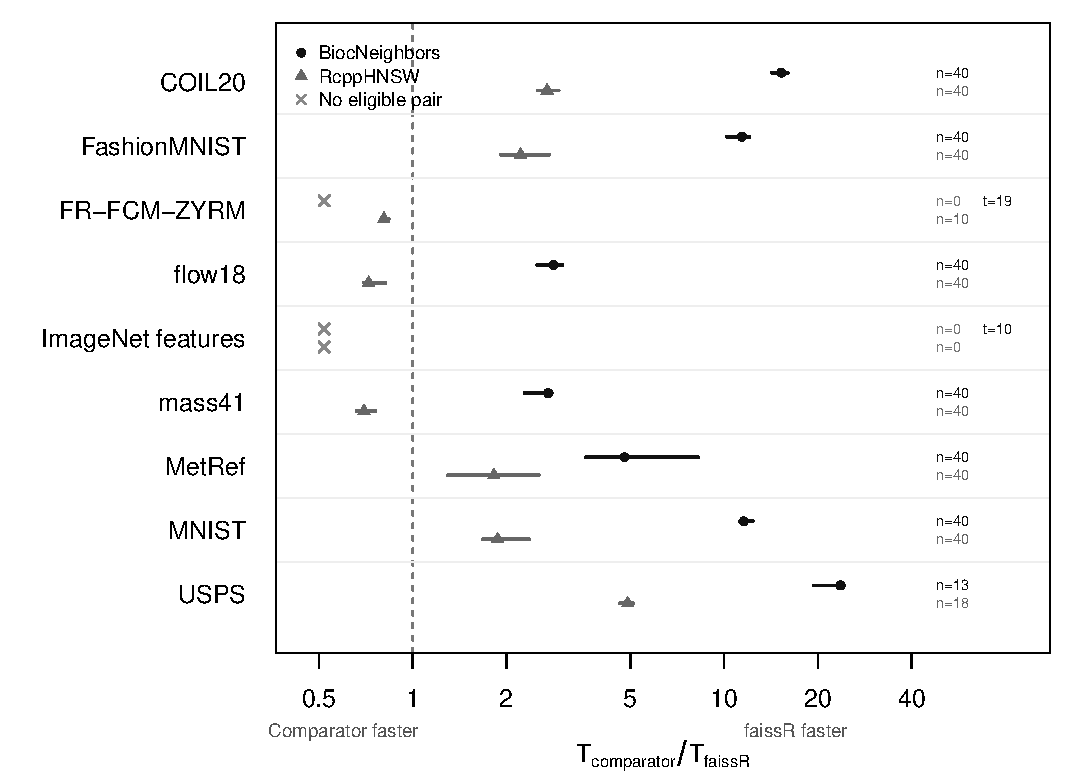
\includegraphics[width=\textwidth]{fig_paired_cpu_log_ratio.pdf}
\caption{Secondary controlled CPU HNSW cold-call evidence for prespecified
public configurations. Points are dataset medians and horizontal lines are
interquartile intervals among pairs for which both routes had mean recall at
least 0.99 in every included replicate. Ratios are
$T_{\mathrm{comparator}}/T_{\mathrm{faissR}}$ on a logarithmic axis. Black
circles and grey triangles distinguish the two comparators in grayscale;
crosses denote no mean-recall-matched pair. The aligned right-hand columns
show the number of eligible pairs (\code{n}) and timeout counts (\code{t}) among 40
planned pairs per dataset and comparator.
The providers were not independently tuned, active threads were not observed,
and the conditional ratios are not provider-level speed estimates.}
\label{fig:supp-paired-cpu}
\end{figure}

\subsection{Independently tuned HNSW}

This experiment varied search effort for every dataset--$k$ combination and
construction effort at $k=30$. Each provider was tuned separately. Among
configurations with mean recall of at least 0.99 in all three calibration
repetitions, the fastest was selected and evaluated over five repetitions on
independent queries. Cold-call, index-build, and fitted-query times were
measured separately. A phase-specific ratio was reported only when both
providers met the same mean-recall threshold in every validation repetition.
Table 5 of the main article reports the eligible counts and phase-specific
median ratios.

Both interfaces received the same R double matrix. Conversion to the float32
representation required by FAISS was included in the timed \pkg{faissR}
call; the comparators' internal precision was not instrumented. Calls
requested $k+1$ neighbors and removed the known source row within the timer:
\pkg{faissR} did so in compiled code, while comparator wrappers did so in R.
Provider-returned ordering was retained. The timings cover each complete
public interface, including its result handling.

Twelve threads were requested through the public interfaces. Thread controls
included Open Multi-Processing (OpenMP), OpenBLAS, and the Intel Math Kernel
Library (MKL), through \code{OMP\_NUM\_THREADS},
\code{OPENBLAS\_NUM\_THREADS}, and \code{MKL\_NUM\_THREADS}. The run recorded
the Slurm allocation, Linux affinity mask, these variables, and process-thread
counts before and after each call. They document requested limits and observed
process counts; active internal workers may still differ among providers.
\subsection{Seven-package comparison}

The broader comparison included \pkg{FNN}, \pkg{RANN}, \pkg{Rnanoflann},
\pkg{BiocNeighbors}, \pkg{RcppHNSW}, \pkg{RcppAnnoy}, and \pkg{rnndescent}.
All 216 tasks returned recorded outcomes: 6,480 route repetitions, including
1,385 timeouts and 22 other failures. Of 4,104 planned paired repetitions,
2,866 completed successfully for both methods, and 1,636 also met the requested
mean-recall tier. Table 6 of the main article reports the class-level ratios,
eligibility counts, and timeout totals for the same-family and task-level
comparisons. It excludes the experimental derived-route comparison.
Figure~\ref{fig:supp-comprehensive-r} shows all dataset medians and their
across-dataset summaries. Dataset-specific values appear in
Table~\ref{tab:supp-comprehensive-datasets}.

The comparison respects the metrics and input types accepted by each public
interface. Exact and HNSW interfaces were paired with the corresponding
\pkg{faissR} families. Annoy interfaces were paired with
\code{method = "auto"} as task-level alternatives because \pkg{faissR} does
not implement Annoy. The \pkg{rnndescent} comparison uses the experimental,
noncanonical \code{nndescent\_style} route and is reported here only as
descriptive evidence. Shared \pkg{faissR} calls can contribute to several
comparator pairs, so the timeout totals overlap across classes.
\begin{table}[H]
\centering
\scriptsize
\begin{tabularx}{\textwidth}{@{}l*{4}{>{\centering\arraybackslash}X}@{}}
\toprule
\multicolumn{5}{@{}l}{\textit{Panel A: same-family exhaustive comparisons}} \\
\addlinespace[0.25em]
Dataset & \pkg{FNN} exact & \pkg{RANN} exact & \pkg{Rnanoflann} exact & \pkg{BiocNeighbors} exact \\
\midrule
COIL-20 & 32.00 (72) & 37.69 (48) & 8.60 (24) & 4.73 (48) \\
Fashion-MNIST & -- & -- & 22.04 (24) & 15.33 (48) \\
FR-FCM-ZYRM & -- & -- & -- & -- \\
MNIST & -- & -- & 21.35 (24) & 15.40 (48) \\
MetRef & 4.24 (72) & 6.63 (48) & 2.31 (24) & 2.21 (48) \\
USPS & 37.80 (45) & 40.73 (18) & 9.00 (18) & 3.16 (36) \\
flow18 & -- & -- & -- & 2.06 (6) \\
ImageNet features & -- & -- & -- & -- \\
mass41 & -- & -- & -- & 1.97 (4) \\
\midrule
\multicolumn{5}{@{}l}{\textit{Panel B: same-family HNSW comparisons}} \\
\addlinespace[0.25em]
Dataset & \multicolumn{2}{c}{\pkg{BiocNeighbors} HNSW} & \multicolumn{2}{c}{\pkg{RcppHNSW} HNSW} \\
\midrule
COIL-20 & \multicolumn{2}{c}{11.58 (48)} & \multicolumn{2}{c}{2.61 (48)} \\
Fashion-MNIST & \multicolumn{2}{c}{9.84 (42)} & \multicolumn{2}{c}{1.67 (48)} \\
FR-FCM-ZYRM & \multicolumn{2}{c}{--} & \multicolumn{2}{c}{0.75 (12)} \\
MNIST & \multicolumn{2}{c}{8.88 (48)} & \multicolumn{2}{c}{1.68 (48)} \\
MetRef & \multicolumn{2}{c}{5.19 (48)} & \multicolumn{2}{c}{6.60 (48)} \\
USPS & \multicolumn{2}{c}{13.36 (17)} & \multicolumn{2}{c}{3.95 (17)} \\
flow18 & \multicolumn{2}{c}{2.98 (48)} & \multicolumn{2}{c}{0.78 (48)} \\
ImageNet features & \multicolumn{2}{c}{--} & \multicolumn{2}{c}{--} \\
mass41 & \multicolumn{2}{c}{2.78 (48)} & \multicolumn{2}{c}{0.73 (48)} \\
\midrule
\multicolumn{5}{@{}l}{\textit{Panel C: task-level Annoy alternatives}} \\
\addlinespace[0.25em]
Dataset & \multicolumn{2}{c}{\pkg{BiocNeighbors} Annoy / \pkg{faissR} auto} & \multicolumn{2}{c}{\pkg{RcppAnnoy} / \pkg{faissR} auto} \\
\midrule
COIL-20 & \multicolumn{2}{c}{1.57 (48)} & \multicolumn{2}{c}{1.68 (48)} \\
flow18 & \multicolumn{2}{c}{1.89 (45)} & \multicolumn{2}{c}{2.62 (41)} \\
mass41 & \multicolumn{2}{c}{1.36 (3)} & \multicolumn{2}{c}{--} \\
\midrule
\multicolumn{5}{@{}l}{\textit{Panel D: experimental derived-route comparison}} \\
\addlinespace[0.25em]
Dataset & \multicolumn{4}{c}{\pkg{rnndescent} NN-descent / \pkg{faissR} \code{nndescent\_style}} \\
\midrule
COIL-20 & \multicolumn{4}{c}{0.22 (72)} \\
MetRef & \multicolumn{4}{c}{1.30 (72)} \\
USPS & \multicolumn{4}{c}{0.73 (36)} \\
\bottomrule
\end{tabularx}
\caption{Dataset medians for the seven-package comparison. Entries are median
$T_{\mathrm{comparator}}/T_{\mathrm{faissR}}$ followed by the number of
eligible paired repetitions in parentheses. A dash indicates that the dataset
had no pair in which both methods completed and met the requested mean recall.
Panels A and B are same-family comparisons. Panel C compares task-level
alternatives, not Annoy implementations. Panel D is an experimental
derived-route comparison and is excluded from the principal performance
table.}
\label{tab:supp-comprehensive-datasets}
\end{table}

\begin{figure}[h]
\centering
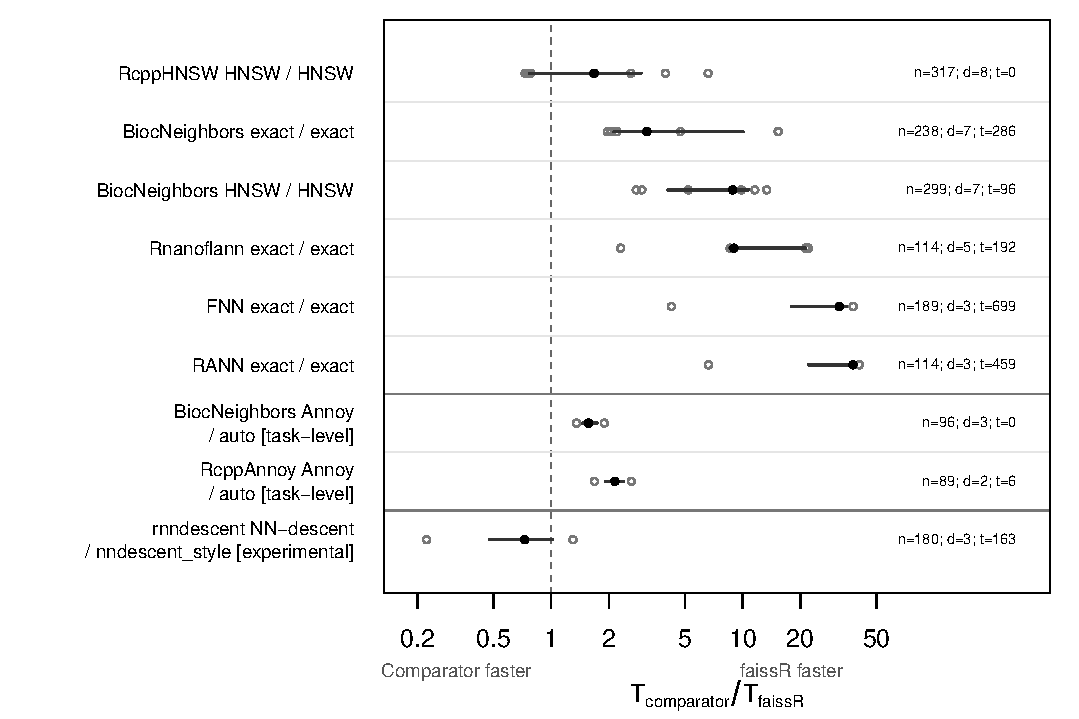
\includegraphics[width=0.94\textwidth]{fig_comprehensive_r_log_ratio.pdf}
\caption{Complete matched-node public-interface CPU comparison in grayscale.
Open circles are the medians of eligible repetition-level ratios within each
dataset. Solid points and bars are the median and interquartile interval of
those dataset medians. Right labels give matched-pair counts (\code{n}),
datasets with at least one matched pair (\code{d}), and total timeouts
(\code{t}) in each comparator class. Each y-axis label gives the
external package and method, followed after the slash by the matched
\pkg{faissR} method. Task-level and experimental comparisons are marked in
their labels. Ratios describe the prespecified public configurations.}
\label{fig:supp-comprehensive-r}
\end{figure}

\section{Query batches and index reuse}
\label{sec:supp-workload}

The query-workload experiment used five datasets and external batches of 1,
32, and up to 1,024 queries. It recorded cold and warm calls after clearing
the package cache at the start of each sequence. The difference
$\max(T_{\mathrm{cold}}-T_{\mathrm{warm}},0)$ estimates setup cost; it is not
a separately instrumented index-build time. For $A$ batches, the estimated
total was $T_{\mathrm{cold}}+(A-1)T_{\mathrm{warm}}$, evaluated at
$A\in\{1,10,100\}$.

All 60 CPU and 60 CUDA cells completed. CPU HNSW reused a fitted index in all
15 HNSW cells. For 13 of these, reuse became faster than repeating cold Flat
calls within the evaluated range. The break-even point is the smallest $A$
satisfying
\[
T_{\mathrm{cold},M}+(A-1)T_{\mathrm{warm},M}
\leq A\,T_{\mathrm{cold},\mathrm{Flat}}.
\]
Among the 13 cases that reached break-even, the median smallest $A$ was 13
query batches. The Flat baseline rebuilt its index for every call, so this is
not a comparison with a reusable exact index. All 60 CUDA cells reported zero
index-cache hits. The observed reuse benefit therefore applies to the CPU
experiment.

GPU-resident output was assessed through interface, ownership, and explicit
transfer tests. Transfer speed, downstream consumer performance, and
quantitative host- or device-memory comparisons remain unmeasured.
Process-lifetime memory high-water marks cannot establish per-cell peak memory
when several cells share a worker.

\section{Experiment completion}

Table~\ref{tab:supp-evidence-audit} collects the completion and quality checks
used in the article. A completed execution is not necessarily a
target-attaining result: calibration recommendations below target and
comparator calls below the mean-recall threshold remain in the raw files.
The summary also includes the leave-one-dataset-out (LOODO) reconstruction.
Likewise, recorded outcomes include failures and timeouts, not only successful
calls. The table keeps those denominators separate.

\begin{table}[h]
\centering

\begin{tabularx}{\textwidth}{@{}Yrr@{}}
\toprule
Evidence & Passing or completed & Total \\
\midrule
CPU route-contract cells & 48 & 48 \\
CUDA route-contract cells & 52 & 52 \\
Public-metric reference records & 87 & 87 \\
Completed calibration operating points & 6,453 & 6,804 planned \\
Approximate calibration targets met & 3,653 & 4,725 completed \\
CUDA automatic independent-query cells & 324 & 324 \\
CPU HNSW independent-query cells & 304 & 324 \\
CUDA LOODO operating-point cells & 324 & 324 \\
CUDA LOODO method-family agreement & 300 & 324 \\
CPU LOODO operating-point cells & 301 & 324 \\
CPU LOODO method-family agreement & 292 & 313 evaluable \\
CPU LOODO abstentions & 4 & 324 \\
Controlled CPU HNSW route pairs & 720 & 720 \\
Successful controlled CPU HNSW pairs & 691 & 720 \\
Independently tuned HNSW route runs & 720 & 720 \\
Independently tuned HNSW target-matched provider pairs & 63 & 72 \\
CPU query-workload cells & 60 & 60 \\
CUDA query-workload cells & 60 & 60 \\
Comprehensive CPU comparison tasks & 216 & 216 \\
Comprehensive CPU paired repetitions & 4,104 & 4,104 \\
Comprehensive mean-recall-matched pairs & 1,636 & 4,104 \\
\bottomrule
\end{tabularx}
\caption{Evidence used by the article.}
\label{tab:supp-evidence-audit}
\end{table}

\section{CUDA selection and sensitivity analyses}
\label{sec:supp-selector}

The bundled CUDA selector is an experimental L40S-calibrated policy for cold
full self-search. It selected Flat in 280 of 324 cells and IVF in 44; all
selected routes met their eligibility criterion. CPU automatic selection has
not been independently validated and is labelled
\path{auto_policy_status=calibration_informed_not_independently_validated}
and \path{auto_policy_evidence_scope=cpu_static_policy_experimental}.
CUDA results record the narrower scope \code{cuda\_cold\_full\_self\_search}.

A device model other than the L40S, or an unidentified model, is marked
\path{hardware_extrapolated_unvalidated} and triggers a once-per-model
session warning, which users can disable after inspection. The policy is
not silently replaced. Local \code{pilot} and \code{cache} tuning search
within a chosen method; they do not create a new cross-method policy.
The selector does not accept a memory budget, build-time or latency limit,
or a constraint forbidding exhaustive search. Users who need such limits
must choose and assess an explicit method.

\subsection{Validation and route choices}

Two query seeds defined independent audit samples from each named dataset.
Each seed sampled $\min(n,1024)$ rows uniformly without replacement,
including all 873 rows of MetRef. Calls timed full self-search; recall was
computed only on the sampled rows. Three execution repeats reused each
sample and recomputed identifier-overlap recall. Approximate routes had to
reach the requested mean recall in every repeat under both seeds.
These repeats assess runtime and execution stability, not six independent
query samples. The samples also share the reference matrix.

Neither calibration nor validation used a confidence-bound eligibility
criterion. No query-bootstrap lower bounds were available for these results.
Alternative identifiers at tied boundaries can reduce approximate overlap;
this effect was not quantified. Exact-family routes instead passed the
separate distance-based audit. These distinctions matter when applying the
results to rare populations or a different query distribution.

By metric, Flat/IVF counts were 64/44 for Euclidean, 108/0 for cosine, and
108/0 for correlation. By target they were 92/16 at 0.90, 92/16 at 0.95,
and 96/12 at 0.99. Each value of $k$ contributed 81 cells, with 70 Flat and
11 IVF selections. Table~\ref{tab:supp-auto-routes} gives the dataset counts.

\begin{table}[h]
\centering

\begin{tabularx}{\textwidth}{@{}Xrr@{}}
\toprule
Dataset & Flat & IVF \\
\midrule
COIL20 & 36 & 0 \\
FashionMNIST & 36 & 0 \\
FR-FCM-ZYRM & 24 & 12 \\
flow18 & 24 & 12 \\
ImageNet features & 28 & 8 \\
mass41 & 24 & 12 \\
MetRef & 36 & 0 \\
MNIST & 36 & 0 \\
USPS & 36 & 0 \\
\bottomrule
\end{tabularx}
\caption{CUDA automatic route selections by dataset. Each row contains 36
metric--$k$--target cells.}
\label{tab:supp-auto-routes}
\end{table}

The selected IVF parameters are listed in
Table~\ref{tab:auto-ivf-parameters}. Across 108 dataset--metric--$k$
combinations, changing the requested tier changed the method in four,
changed parameters without changing method in six, and changed neither in
98. The effect was concentrated in large Euclidean problems. For the
low-dimensional datasets, numeric parameters changed at $k=15$ and $k=30$,
but not at $k=50$ or $k=100$. ImageNet switched to Flat at target 0.99.

Probe counts obey $1\leq\code{nprobe}\leq\code{nlist}$. For example,
308 of 5,898 lists is about 5.2\%, and 160 of 1,590 is about 10.1\%.
These settings were feasible on the 48-gigabyte L40S. Users of smaller GPUs
should assess an explicit configuration because lowering \code{nprobe} would
change the selected operating point.

\begin{table}[h]
\centering

\begin{tabularx}{\textwidth}{@{}Xrrrr@{}}
\toprule
Shape represented in evaluation & $k$ & 0.90 & 0.95 & 0.99 \\
\midrule
Large low-dimensional & 15 & (512, 6) & (512, 6) & (512, 12) \\
Large low-dimensional & 30 & (512, 6) & (1024, 16) & (1024, 32) \\
Large low-dimensional & 50 & (1966, 90) & (1966, 90) & (1966, 90) \\
Large low-dimensional & 100 & (5898, 308) & (5898, 308) & (5898, 308) \\
ImageNet features & 15 & (1590, 160) & (1590, 160) & Flat \\
ImageNet features & 30 & (1060, 99) & (1060, 99) & Flat \\
ImageNet features & 50 & (1590, 160) & (1590, 160) & Flat \\
ImageNet features & 100 & (1590, 160) & (1590, 160) & Flat \\
\bottomrule
\end{tabularx}
\caption{Selected CUDA IVF parameters as $(\code{nlist},\code{nprobe})$.
``Flat'' indicates a target-dependent route change.}
\label{tab:auto-ivf-parameters}
\end{table}

\subsection{Regret and runtime comparisons}

Regret is selected-route time divided by the fastest eligible observed route
time, including the selected route itself. Exact-audited methods are eligible
by the exhaustive audit; approximate methods must meet the requested mean
recall in every validation repeat. Table~\ref{tab:selector-regret-dataset}
compares the installed policy with a post hoc cross-fitted reconstruction.
Each analysis contains 324 selected cells and 1,944 successful executions,
with no selected-route failure, timeout, or memory kill.

The two analyses use different candidate sets. The installed policy chose
Flat or IVF, whereas the complete explicit routes available for
cross-fitting were exact-family methods and CAGRA; explicit IVF was absent.
The cross-fitted results are therefore a candidate-set sensitivity analysis.
The table's net time difference is
$T_{\mathrm{exact}}-T_{\mathrm{selected}}$, summed across the 36
metric--$k$--target combinations for each dataset. It describes this benchmark,
not savings weighted by an external application's workload.

\begin{table}[h]
\centering

\small
\setlength{\tabcolsep}{4pt}
\begin{tabular}{@{}lrrr@{\hspace{5mm}}rrr@{}}
\toprule
& \multicolumn{3}{c}{Experimental installed policy} & \multicolumn{3}{c}{Post hoc sensitivity} \\
\cmidrule(lr){2-4}\cmidrule(lr){5-7}
Dataset & \shortstack{Median\\regret} & \shortstack{Approximate\\faster} & \shortstack{Net\\seconds} & \shortstack{Median\\regret} & \shortstack{Approximate\\faster} & \shortstack{Net\\seconds} \\
\midrule
COIL20 & 1.14 & -- & $-0.6$ & 1.00 & -- & $2.4$ \\
FashionMNIST & 1.02 & -- & $-0.7$ & 1.00 & -- & $0.2$ \\
FR-FCM-ZYRM & 1.63 & 12/12 & $3317.7$ & 1.00 & 9/9 & $6561.5$ \\
MNIST & 1.01 & -- & $-0.4$ & 1.00 & -- & $0.3$ \\
MetRef & 1.48 & -- & $-0.7$ & 1.00 & -- & $2.5$ \\
USPS & 1.33 & -- & $-0.5$ & 1.00 & -- & $2.5$ \\
flow18 & 1.88 & 12/12 & $141.2$ & 1.00 & 12/12 & $290.4$ \\
ImageNet features & 1.00 & 0/8 & $-8001.1$ & 1.00 & -- & $33.1$ \\
mass41 & 1.88 & 12/12 & $128.8$ & 1.00 & 12/15 & $264.2$ \\
\bottomrule
\end{tabular}
\caption{CUDA selector regret and absolute time difference by dataset under the
cold full-self-search workload.}
\label{tab:selector-regret-dataset}
\end{table}

Cell-level regret and route choices are supplied in
\path{jss_selector_regret_cells.csv},
\path{jss_selector_regret_by_stratum.csv}, and
\path{jss_selector_route_choices.csv}. They describe one workload,
\code{cold\_full\_self\_search}. The 324 cells are nested within nine datasets
and are not 324 independent experimental units.

The complete CUDA comparison contained automatic selection, explicit exact
Flat, brute force, and CAGRA, each with 1,944 successful executions. Every
timed call used \code{nn()} and returned host-resident matrices. The CPU
explicit HNSW set also contained 1,944 successful executions.
Table~\ref{tab:supp-cuda-paired} summarizes CUDA ratios across datasets;
Table~\ref{tab:supp-cuda-dataset} shows their heterogeneity. Among the 44
IVF selections, 36 were faster than explicit exact search. The median
dataset-level ratio for IVF-selected cells was 4.59, but the ImageNet
ratio of 0.14 favored exact search.

\begin{table}[ht]
\centering
\small

\begin{tabularx}{\textwidth}{@{}Xlrrr@{}}
\toprule
Comparison & Datasets & Median & IQR & Range \\
\midrule
Automatic / explicit exact & 9 & 0.99 & 0.98--1.00 & 0.94--1.01 \\
Automatic / brute force & 9 & 0.87 & 0.83--1.18 & 0.70--1.90 \\
Automatic / CAGRA & 9 & 2.23 & 1.00--2.58 & 0.81--10.96 \\
IVF-selected / explicit exact & 4 & 4.59 & 2.80--5.58 & 0.14--5.83 \\
\bottomrule
\end{tabularx}
\caption{Secondary matched CUDA end-to-end ratios. Each ratio is
\(T_{\mathrm{second\ route}}/T_{\mathrm{automatic}}\), so values above one
favor automatic selection. Dataset medians are summarized across datasets.}
\label{tab:supp-cuda-paired}
\end{table}

\begin{table}[ht]
\centering
\small

\setlength{\tabcolsep}{3.2pt}
\begin{tabular}{@{}lrrrrrr@{}}
\toprule
Dataset & Auto target & Exact/auto & Brute/auto & CAGRA/auto & IVF target & Exact/IVF \\
\midrule
COIL20 & 36/36 & 0.98 & 0.87 & 1.00 & 0/0 & -- \\
FashionMNIST & 36/36 & 0.98 & 1.18 & 10.94 & 0/0 & -- \\
FR-FCM-ZYRM & 36/36 & 1.00 & 1.00 & 0.81 & 12/12 & 3.69 \\
MNIST & 36/36 & 0.99 & 1.18 & 10.96 & 0/0 & -- \\
MetRef & 36/36 & 0.94 & 0.70 & 2.40 & 0/0 & -- \\
USPS & 36/36 & 0.96 & 0.75 & 2.58 & 0/0 & -- \\
flow18 & 36/36 & 1.00 & 0.83 & 0.96 & 12/12 & 5.83 \\
ImageNet features & 36/36 & 1.01 & 1.90 & 2.23 & 8/8 & 0.14 \\
mass41 & 36/36 & 1.00 & 0.85 & 1.00 & 12/12 & 5.49 \\
\bottomrule
\end{tabular}
\caption{CUDA results by dataset. Automatic validation attainment covers 36
metric--$k$--target cells. All routes completed without timeout. Ratios use
second-route time divided by automatic-route time. The last ratio is restricted
to cells in which automatic selection chose IVF; values above one favor IVF.
Ratio entries are dataset medians of matched replicate ratios.}
\label{tab:supp-cuda-dataset}
\end{table}

\subsection{Dataset and domain holdouts}

The leave-one-dataset-out (LOODO) reconstruction removed every calibration
row belonging to the held-out dataset. It selected a method using the same
prespecified shape group where possible, or the three nearest training
datasets in $\log(n)$--$\log(p)$ space otherwise. The omitted dataset was
used only for evaluation. CUDA selected an exact-audited family in 288 cells
and CAGRA in 36, with no abstentions. Median regret was 1.00, the 90th
percentile was 1.00, and the range was 1.00--2.24. Method-family agreement
with the empirical oracle was 300/324. Pairwise and joint comparisons with
the installed policy are in
\path{jss_leave_one_dataset_out_route_confusion.csv} and
\path{jss_leave_one_dataset_out_route_joint.csv}.

Holding out an entire domain gave less favorable results
(Table~\ref{tab:supp-domain-holdout}). In particular, the cytometry holdout
had median regret 3.08 and a 95th percentile of 6.93. This shows why removing
one named dataset may be a weak test when related datasets remain in the
collection. The grouped analysis covers three domains and the same explicit
candidate set; its scope ends at the observed hardware, geometries, and shape
range.

\begin{table}[ht]
\centering
\small

\begin{tabular}{@{}lrrrrrr@{}}
\toprule
Held-out domain & Datasets & Cells & Target met & Oracle agreement & Median & 95th percentile \\
\midrule
Image-derived & 5 & 180 & 176 & 153 & 1.06 & 6.19 \\
Cytometry & 3 & 108 & 108 & 66 & 3.08 & 6.93 \\
Metabolomics & 1 & 36 & 36 & 36 & 1.00 & 1.00 \\
\bottomrule
\end{tabular}
\caption{Grouped leave-one-domain-out sensitivity reconstructed from the
available explicit independent-query CUDA routes. Regret is selected-route time divided
by empirical-oracle time.}
\label{tab:supp-domain-holdout}
\end{table}

The analogous CPU reconstruction attained 301/324 operating points and
abstained in four. It agreed with the oracle method family in 292/313
evaluable cells. HNSW was selected in 309 cells and exact search in 15;
11 exact selections passed the held-out exactness audit. Median regret was
1.00, the 90th percentile was 1.00, and the range was 1.00--3.16.
These results apply to the reconstructed policy; installed CPU \code{auto}
was evaluated separately. The replication directory \path{cpu_loodo/} contains all 324
rows, dataset and metric summaries, the audit report, and checksum ledger.

\section{Replication}

The replication bundle provides the source package, reference manual,
vignette, practical CPU example, and a single commented article script with
HyperText Markup Language (HTML) output. It includes checksummed results,
software and dataset fingerprints, and the files needed to reconstruct the
tables and figures.

The script has three modes. \code{compact} runs the interface example on an
ordinary CPU computer. \code{archive} verifies checksums before extraction
and reconstructs numerical summaries from the stored results.
\code{all} runs both. Archive reanalysis runs on CPU; repeating the CUDA
experiments requires compatible NVIDIA hardware and the recorded
FAISS/cuVS build. A checksum, schema, dataset-fingerprint, aggregation, or
table-audit failure stops execution. A successful run records verification
results, per-table SHA-256 digests, and a fresh \code{sessionInfo.txt}.

The archive table builder produces 18 numerical summaries with stable file
identifiers, which are not article table numbers. Separate checksum-verified
inputs reconstruct the controlled CPU figures, seven-package comparison,
tuned HNSW results, and query-workload results. Interface and installation
tables summarize software contracts and tested environments.
The bundle is a checksummed snapshot; a persistent archival identifier is
not yet available.

\bibliographystyle{plain}
\bibliography{faissR_jss}

\end{document}
